\section*{Analiza porównawcza spójności wyjaśnień}

W tej sekcji przeprowadzono ocenę spójności wyjaśnień generowanych przez różne metody XAI: LIME, SHAP i GradCAM.
Celem analizy było zrozumienie, jak bardzo wyjaśnienia nakładają się na siebie oraz jak różne techniki identyfikują istotne cechy obrazu.
Zrozumienie spójności jest kluczowe, gdyż pozwala ocenić, które metody są zgodne w identyfikowaniu obszarów istotnych dla predykcji modeli.

Spójność wyjaśnień oceniono za pomocą współczynnika Intersection over Union (IoU) między obszarami wyjaśnień generowanych przez różne metody.
Wysokie wartości IoU wskazują na wysoką zgodność między metodami, natomiast niskie wartości sugerują, że różne metody identyfikują różne obszary jako istotne.

\begin{figure}[h]
	\centering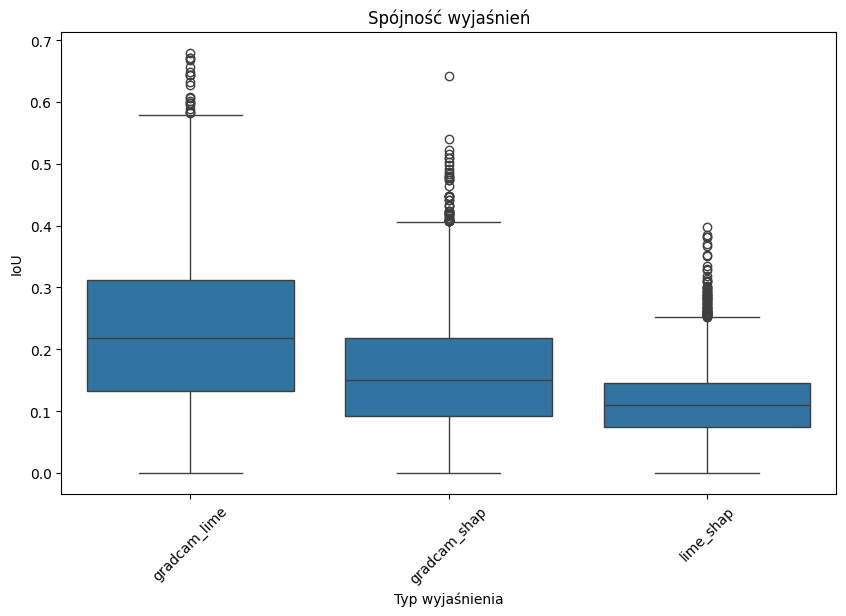
\includegraphics[width=.9\textwidth]{img/base_coherence}
	\caption{Spójność wyjaśnień}  \label{rys:base_coherence}
\end{figure}

\begin{table}[h]
	\centering
	\begin{tabular}{|c|c|}
		\hline
		\textbf{Metody XAI}     & \textbf{Średnie IoU} \\
		\hline
		\textbf{GradCAM i LIME} & 0.178567             \\
		\hline
		\textbf{GradCAM i SHAP} & 0.111023             \\
		\hline
		\textbf{LIME i SHAP}    & 0.072478             \\
		\hline
	\end{tabular}
	\caption{Średnie wartości IoU między typami wyjaśnień}
	\label{tab:base_coherence}
\end{table}

Wyniki analizy zostały przedstawione za pomocą wykresu pudełkowego (Rys \ref{rys:base_coherence}), który ilustruje rozkład wartości IoU dla różnych par metod XAI.
Dodatkowo, Tabela \ref{tab:base_coherence} przedstawia średnich wartości IoU dla poszczególnych par metod.
Na końcu pracy, w Dodatku \ref{app1}, znajdują się przykłady obrazów z zaznaczonymi wyjaśnieniami, co dodatkowo ilustruje różnice i podobieństwa między analizowanymi metodami XAI.
Dodatek ten zawiera przykłady dla wartości IoU bliskich średniej, przykłady odstające pozytywnie oraz negatywnie, co pozwala lepiej zrozumieć metody.

\textbf{GradCAM i LIME} generują najbardziej spójne wyjaśnienia, co jest widoczne w najwyższych i najbardziej rozległych wartościach IoU.
Choć nie są identyczne, mają one tendencje do pokrywania się w kluczowych obszarach decyzyjnych modelu.

\textbf{GradCAM i SHAP} - generują niższe średnie wartości IoU.
Spowodowane to może być różnicą w podejściu do generowania wyjaśnień.

\textbf{LIME i SHAP} - generują najniższe średnie wartości IoU.
Warto jednak zauważyć wartości odstające, gdzie SHAP z LIME osiągnęły wyniki wyższe od GradCAM i SHAP.

\vspace{1cm}

W celu dokładniejszej analizy spójność wygenerowanych wyjaśnień, wyniki podzielono ze względu na kategorie obrazów z bazy danych ImageNet-9.
Analiza została przeprowadzona dla różnych kategorii obrazów, co pozwoliło lepiej zrozumieć, jak poszczególne techniki XAI radzą sobie z różnymi rodzajami obrazów.

\begin{figure}[!h]
	\centering
	\begin{subfigure}[b]{0.3\textwidth}
		\centering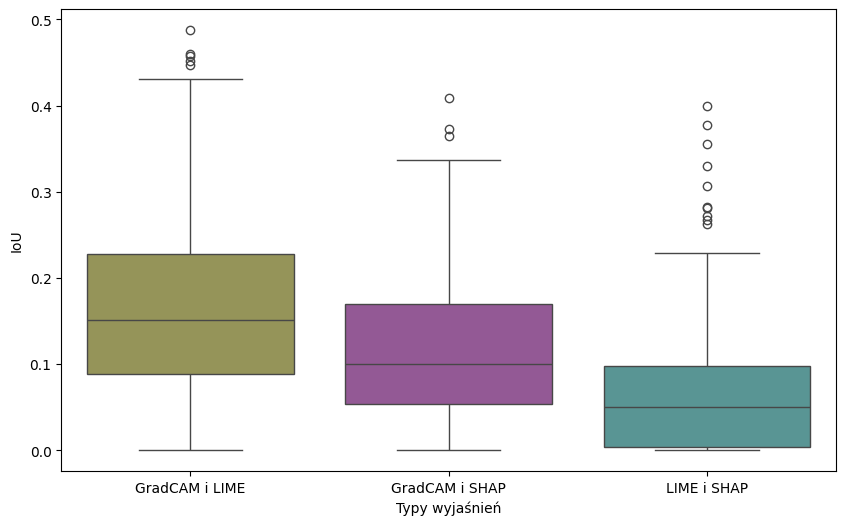
\includegraphics[width=.9\textwidth]{img/base_coherence_dog}
		\caption{Pies}  \label{}
	\end{subfigure}
	\begin{subfigure}[b]{0.3\textwidth}
		\centering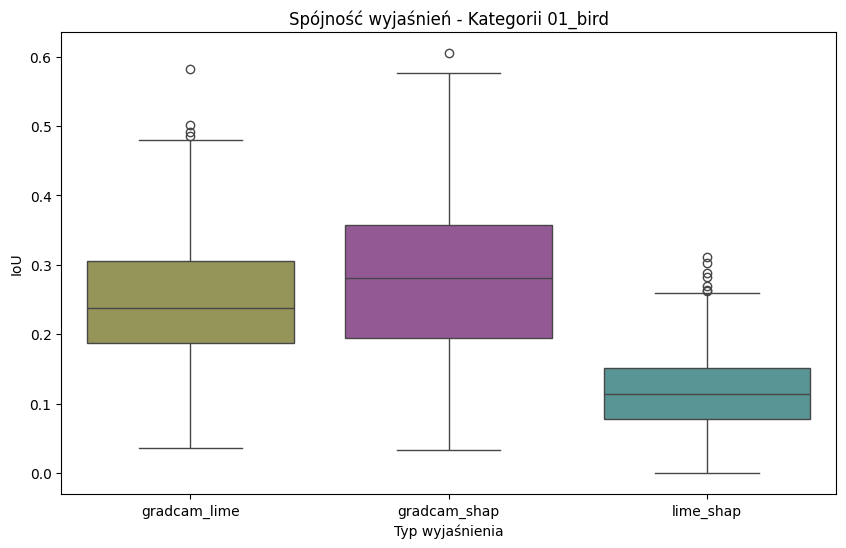
\includegraphics[width=.9\textwidth]{img/base_coherence_bird}
		\caption{Ptak}  \label{}
	\end{subfigure}
	\begin{subfigure}[b]{0.3\textwidth}
		\centering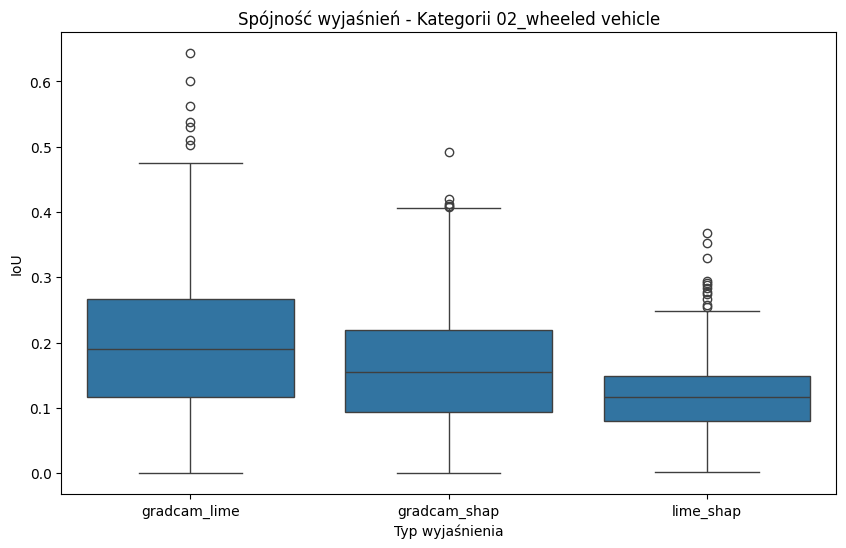
\includegraphics[width=.9\textwidth]{img/base_coherence_vehicle}
		\caption{Pojazd na kołach}  \label{}
	\end{subfigure}
	\begin{subfigure}[b]{0.3\textwidth}
		\centering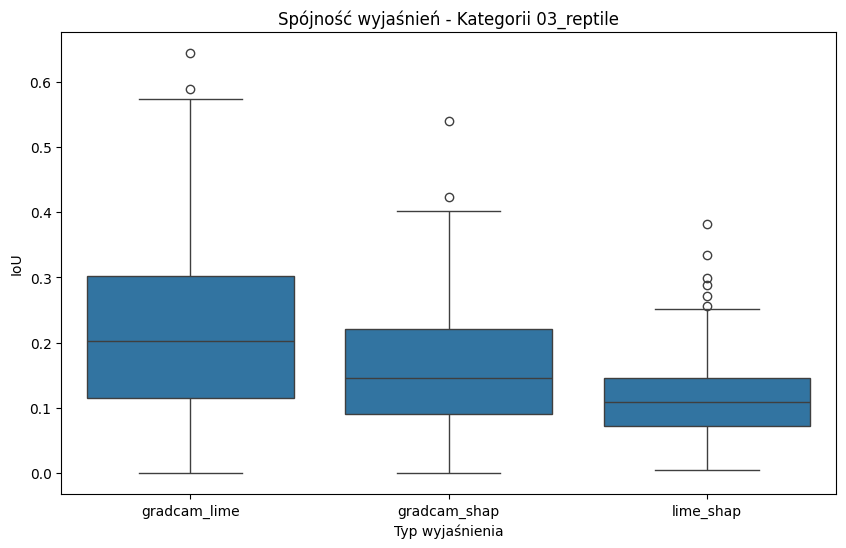
\includegraphics[width=.9\textwidth]{img/base_coherence_reptile}
		\caption{Gad}  \label{}
	\end{subfigure}
	\begin{subfigure}[b]{0.3\textwidth}
		\centering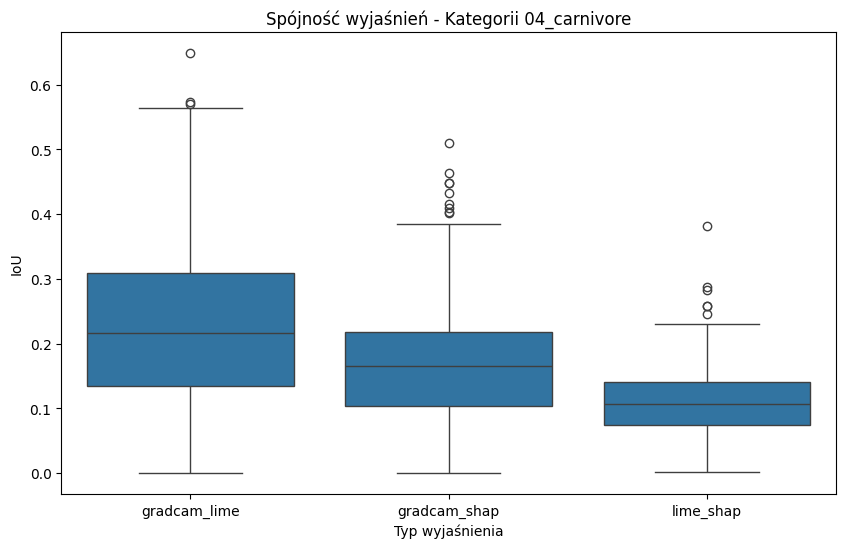
\includegraphics[width=.9\textwidth]{img/base_coherence_carnivore}
		\caption{Mięsożerca}  \label{}
	\end{subfigure}
	\begin{subfigure}[b]{0.3\textwidth}
		\centering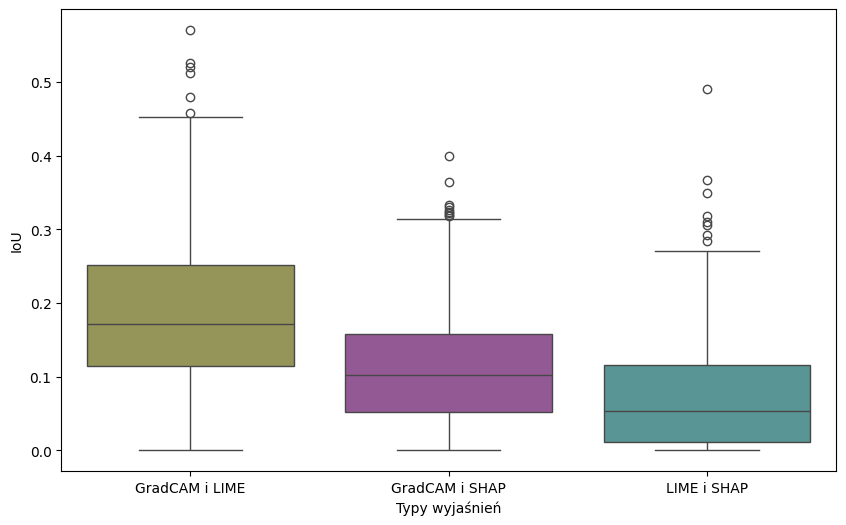
\includegraphics[width=.9\textwidth]{img/base_coherence_insect}
		\caption{Insekt}  \label{}
	\end{subfigure}
	\begin{subfigure}[b]{0.3\textwidth}
		\centering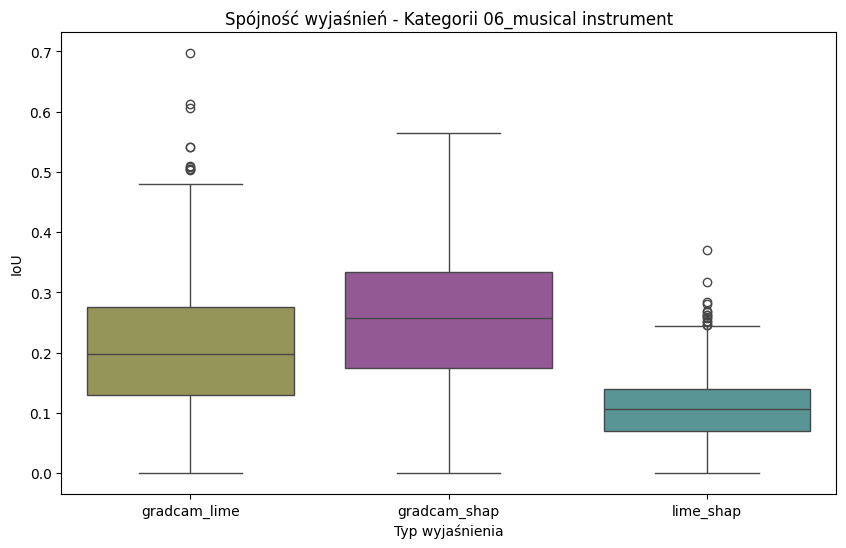
\includegraphics[width=.9\textwidth]{img/base_coherence_music}
		\caption{Instrument muzyczny}  \label{}
	\end{subfigure}
	\begin{subfigure}[b]{0.3\textwidth}
		\centering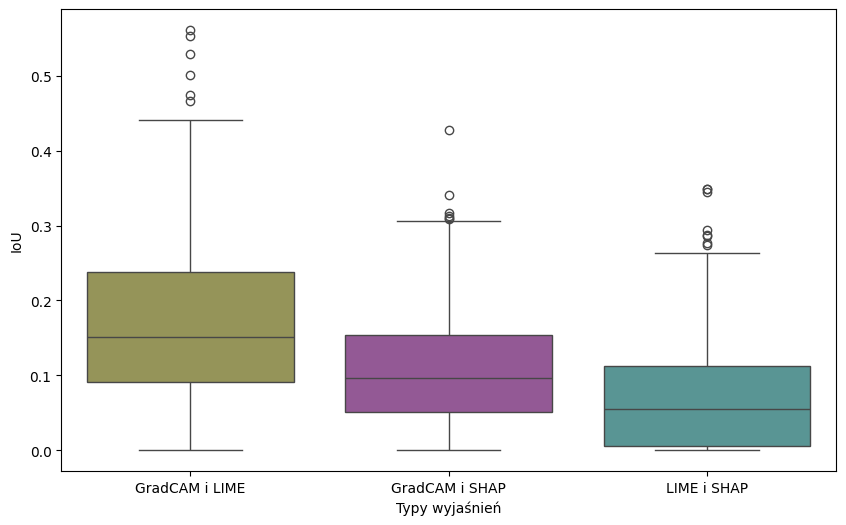
\includegraphics[width=.9\textwidth]{img/base_coherence_primate}
		\caption{Naczelny}  \label{}
	\end{subfigure}
	\begin{subfigure}[b]{0.3\textwidth}
		\centering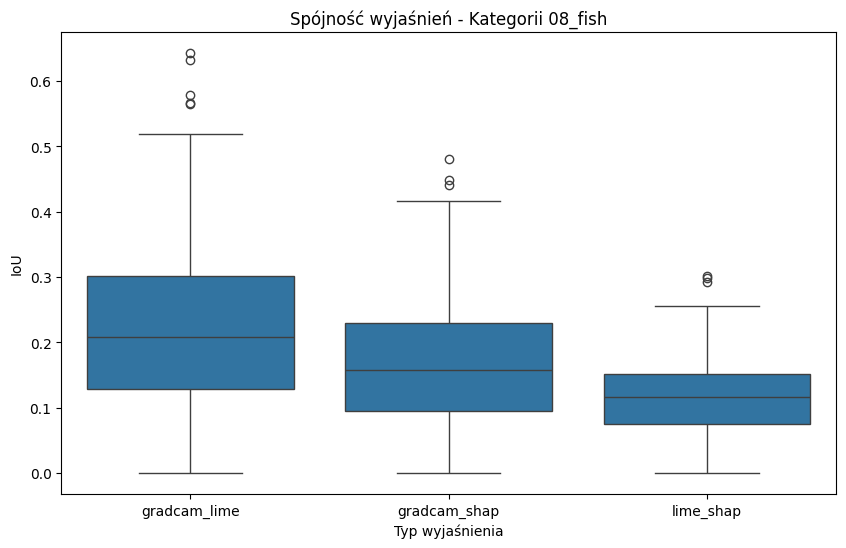
\includegraphics[width=.9\textwidth]{img/base_coherence_fish}
		\caption{Ryba}  \label{}
	\end{subfigure}
	\caption{Spójność wyjaśnień dla różnych kategorii}
	\label{rys:coherence_category}
\end{figure}

\begin{table}[h]
	\centering
	\begin{tabular}{|c|c|c|c|}
		\hline
		\textbf{Kategoria}           & \textbf{GradCAM i LIME} & \textbf{GradCAM i SHAP} & \textbf{LIME i SHAP} \\
		\hline
		\textbf{Pies}                & 0.165114                & 0.113522                & 0.064965             \\
		\hline
		\textbf{Ptak}                & 0.165077                & 0.117948                & 0.075792             \\
		\hline
		\textbf{Pojazd na kołach}    & 0.184504                & 0.109644                & 0.070630             \\
		\hline
		\textbf{Gad}                 & 0.187232                & 0.108796                & 0.077426             \\
		\hline
		\textbf{Mięsożerca}          & 0.167741                & 0.114880                & 0.072844             \\
		\hline
		\textbf{Insekt}              & 0.191125                & 0.112918                & 0.075120             \\
		\hline
		\textbf{Instrument muzyczny} & 0.195389                & 0.100318                & 0.073182             \\
		\hline
		\textbf{Naczelny}            & 0.169974                & 0.107942                & 0.071622             \\
		\hline
		\textbf{Ryba}                & 0.180948                & 0.113242                & 0.070721             \\
		\hline
	\end{tabular}
	\caption{Średnie wartości IoU dla różnych kategorii}
	\label{tab:base_coherence_categories}
\end{table}

Wyniki zostały przedstawione za pomocą wykresu (Rys \ref{rys:coherence_category}) oraz tabeli (Tabela \ref{tab:base_coherence_categories}), które zawierają średnie wartości IoU dla poszczególnych porównań między metodami XAI.

Spójności różnią się w zależności od kategorii, jednak największą spójność zawsze posiada GradCAM z LIME.
Największą spójnością między nimi są kategorie \textit{Instrument muzyczny} oraz \textit{Insekt}.
Z kolei najniższą spójnością dla nich są kategorie \textit{Pies} i \textit{Ptak}.

Najniższą spójnością cechują się zawsze LIME i SHAP, dla których najgorsze wyniki są dla kategorii \textit{Pies}, natomiast najlepsze dla \textit{Gad}.

GradCAM i SHAP posiadają wartości o bliskich wartościach dla wszystkich kategorii.

Kategoria \textit{Insekt} jest jedyną, gdzie średnia wartość IoU dla wszystkich metod XAI jest wyższa niż średnia IoU dla całego zbioru danych, co może sugerować, że te metody lepiej radzą sobie z tego typu obrazami.
Natomiast kategoria \textit{Naczelny} jest jedyną, gdzie średnia wartość IoU dla wszystkich metod XAI jest niższa niż średnia IoU dla całego zbioru danych, co może wskazywać na trudności w identyfikacji istotnych cech przez wszystkie analizowane metody.

\vspace{1cm}
W celu lepszego zrozumienia wpływu wielkości obiektu na spójność wyjaśnień generowanych przez różne metody XAI, podzielono obrazy ze względu na wielkość obiektów.
Badanie miało na celu określenie, czy różne metody XAI identyfikują istotne obszary w sposób zależny od rozmiaru obiektu

\begin{figure}[h]
	\centering
	\begin{subfigure}[b]{0.3\textwidth}
		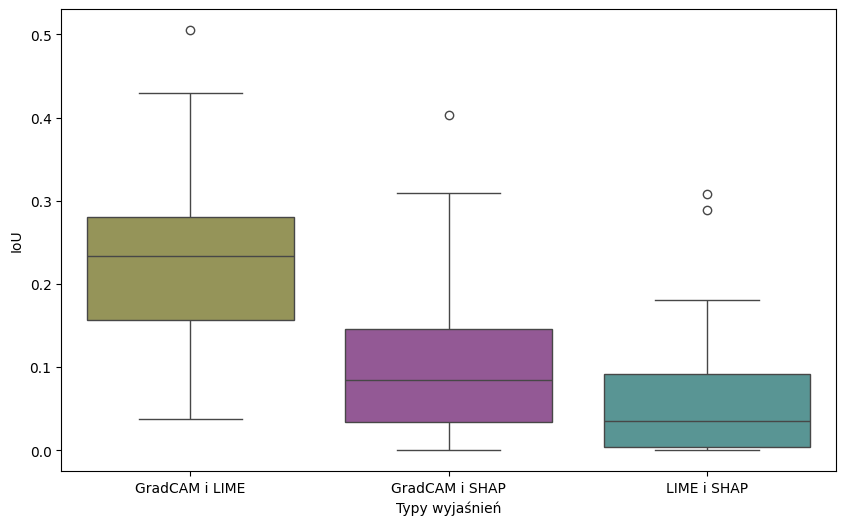
\includegraphics[width=1\textwidth]{img/base_coherence_size_XS}
		\caption{Bardzo mały obiekt}  \label{}
	\end{subfigure}
	\begin{subfigure}[b]{0.3\textwidth}
		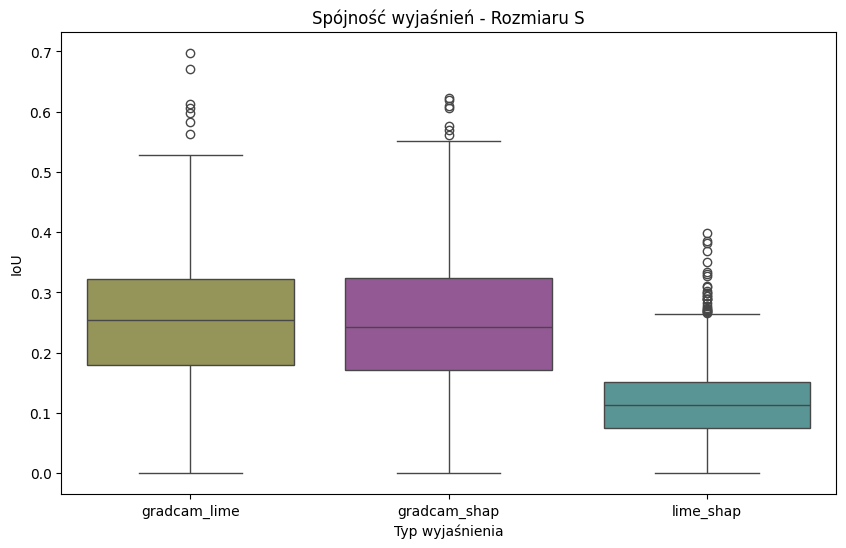
\includegraphics[width=1\textwidth]{img/base_coherence_size_S}
		\caption{Mały obiekt}  \label{}
	\end{subfigure}
	\begin{subfigure}[b]{0.3\textwidth}
		\centering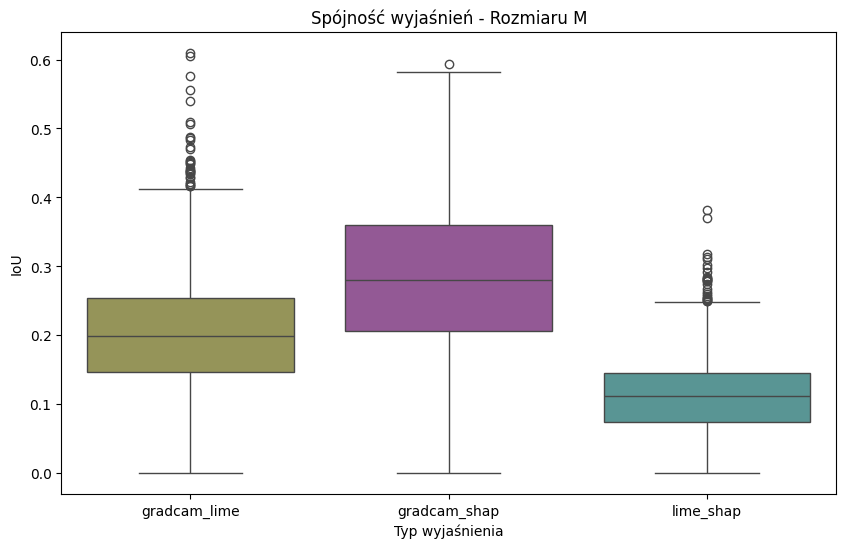
\includegraphics[width=1\textwidth]{img/base_coherence_size_M}
		\caption{Średni obiekt}  \label{}
	\end{subfigure}
	\begin{subfigure}[b]{0.3\textwidth}
		\centering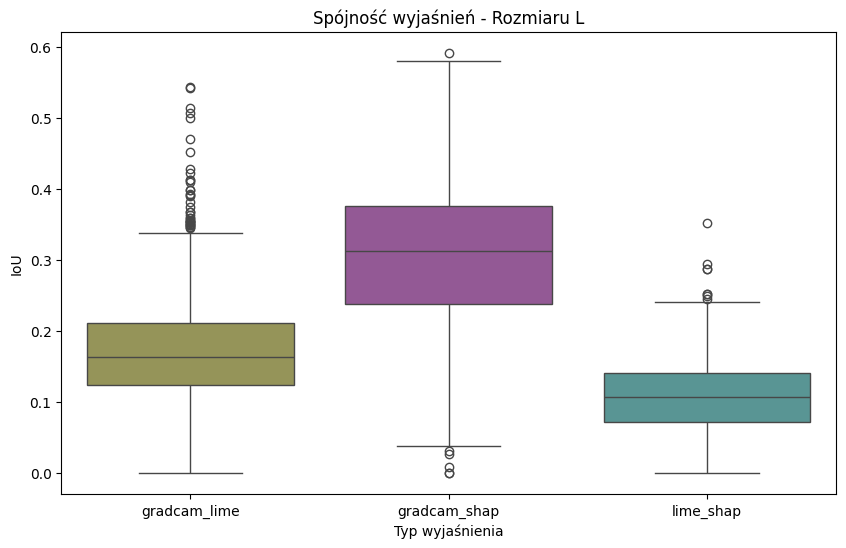
\includegraphics[width=1\textwidth]{img/base_coherence_size_L}
		\caption{Duży obiekt}  \label{}
	\end{subfigure}
	\begin{subfigure}[b]{0.3\textwidth}
		\centering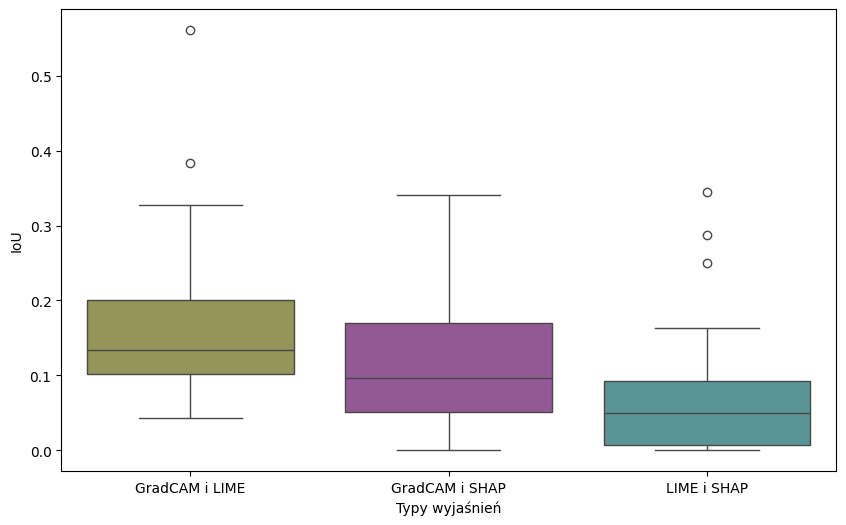
\includegraphics[width=1\textwidth]{img/base_coherence_size_XL}
		\caption{Bardzo duży obiekt}  \label{}
	\end{subfigure}
	\caption{Spójność wyjaśnień dla różnych rozmiarów obiektów}
	\label{rys:coherence_size}
\end{figure}

\begin{table}[h]
	\centering
	\begin{tabular}{|c|c|c|c|}
		\hline
		\textbf{Rozmiar}     & \textbf{GradCAM i LIME} & \textbf{GradCAM i SHAP} & \textbf{LIME i SHAP} \\
		\hline
		\textbf{Bardzo mały} & 0.230775                & 0.106354                & 0.059743             \\
		\hline
		\textbf{Mały}        & 0.191562                & 0.115253                & 0.079477             \\
		\hline
		\textbf{Średni}      & 0.175971                & 0.107933                & 0.068557             \\
		\hline
		\textbf{Duży}        & 0.166485                & 0.110300                & 0.070198             \\
		\hline
		\textbf{Bardzo duży} & 0.163015                & 0.111202                & 0.068941             \\
		\hline
	\end{tabular}
	\caption{Średnie wartości IoU dla różnych rozmiarów}
	\label{tab:base_coherence_size}
\end{table}

Tak jak w poprzednich przypadkach wyniki przedstawiono na wykresie (Rys \ref{rys:coherence_size}) oraz tabeli (Tabela \ref{tab:base_coherence_size}) przedstawiającej średnie wartości IoU dla porównania spójności wyjaśnień w zależności od rozmiaru obiektu na obrazie.

Spójności różnią się w zależności od wielkości obiektu, jednak największą spójność zawsze posiada \textbf{GradCAM z LIME}.
Największą spójność posiadają dla obiektów bardzo małych i ta spójność zmniejsza się wraz ze wzrostem wielkości obiektu.

\textbf{GradCAM i SHAP} największą spójność posiadają dla obiektów małych obiektów, a najmniejszą dla obiektów bardzo małych.
Różnice wynikami dla różnych rozmiarów obiektów są niewielkie.

\textbf{LIME i SHAP} największą spójność posiadają dla obiektów małych, a najmniejszą dla obiektów bardzo małych.

\vspace{1cm}
Analizując te wyniki, można zauważyć, że GradCAM z LIME charakteryzują się wyższą spójnością, natomiast LIME z SHAP charakteryzują się najniższą spójnością.
Może to być spowodowane wielkościami obszarów wyjaśnień, SHAP i LIME mogą oznaczać mniejsze obszary niż GradCAM, co wpływa na ostateczną spójność między nimi.
